%TC: macro \marginfootnote [other]
%TC: envir SCfigure [] other
%TC: macrocount beginSCfigure [figure]
\documentclass[12pt]{report}
\usepackage{preamble}
\setcounter{chapter}{3}
\graphicspath{{../img/}}

\begin{document}
\chapter{Many-body correlations using integral geometry}

This chapter will focus on the morphological framework for the treatment of many-body correlations.
This will cover two related topics:
\begin{enumerate}
\item \emph{Fundamental measure theory} which is ideally suited for correlations in Fourier space i.e.\ structure factors, and
\item The \emph{morphometric approach}, which presents a highly accurate alternative for real space calculations, albeit with many caveats.
\end{enumerate}
These two approaches are related in that they both depend on integral geometry, which we introduced in \ref{sec:integral-geometry}.
In fact, we will see that the latter approach can be seen as a limiting case of the former.
We will focus on the theoretical developments in this chapter, and leave the main body of numerical work to the following chapter where we will apply this to local structure in the hard sphere liquid.

I have tried to make this chapter a relatively self-contained account of the treatment of many-body correlations in hard spheres.
As such there will be a mixture of original results, pure literature review and some original \emph{presentation} of established results.
I will indicate where each of these is the case, though loosely speaking it will start off unoriginal and get progressively more original.
The final sections are entirely original: we use integral geometry to calculate distribution functions in hard spheres, which is work now published as Ref.\ \cite{Robinson2019}.
The results of this chapter only entered the supplementary material of Ref.\ \cite{Robinson2019}, whereas the results of the next chapter were described in the main text.

\section{Functional calculus}

The chain rule of functional calculus is
\todo{Insert citation to some calculus of variations reference, and Hansen2013/Bob's reviews for application to liquids.}
\begin{equation*}
  \frac{\delta f}{\delta u(\vec{r})} =
  \int
  \frac{\delta f}{\delta v(\vec{r}')}
  \frac{\delta v(\vec{r}')}{\delta u(\vec{r})}
  \, d\vec{r}'
\end{equation*}
and inverse derivatives are found via
\begin{equation*}
  \int
  \frac{\delta u(\vec{r})}{\delta v(\vec{r}')}
  \frac{\delta v(\vec{r}')}{\delta u(\vec{r})}
  \, d\vec{r} =
  \delta(\vec{r} - \vec{r}')
\end{equation*}

\section{Fourier transforming weight functions}

\begin{equation}
  \widetilde{\omega}_\alpha(\vec{k}) =
  \int \omega_\alpha (\vec{r}) e^{-i \vec{k}\cdot\vec{r}} \, d\vec{r}
\end{equation}

\begin{align}
  \widetilde{\omega}_3(\vec{k}) &=
  4\pi \frac{\sin{kR} - kR\cos{kR}}{k^3} \\
  \widetilde{\omega}_2(\vec{k}) &=
  4\pi R^2 \frac{\sin{kR}}{kR} \\
  \widetilde{\vec{\omega}}_2(\vec{k}) &=
  - i \vec{k} \widetilde{\omega}_3(\vec{k})
\end{align}

\begin{equation}
  \begin{aligned}
    c_{22}(\vec{r} = \vec{r}_2 - \vec{r}_1) &=
    \frac{1}{(2\pi)^3}
    \iint
    e^{-i (\vec{k}_1\cdot\vec{r}_1 + \vec{k}_2\cdot\vec{r}_2)}
    \widetilde{\omega}_2(\vec{k}_1)
    \widetilde{\omega}_2(\vec{k}_2)
    \delta{(\vec{k}_1 + \vec{k}_2)}
    \, d\vec{k}_1 d\vec{k}_2 \\
    &=
    \frac{1}{(2\pi)^3}
    \int
    e^{i \vec{k}_1 \cdot (\vec{r}_2 - \vec{r}_1)}
    \widetilde{\omega}_2(\vec{k}_1)
    \widetilde{\omega}_2(-\vec{k}_1)
    \, d\vec{k}_1 \\
    &=
    \frac{1}{(2\pi)^3}
    \int
    e^{i \vec{k} \cdot \vec{r}}
    \widetilde{\omega}_2(\vec{k})^2
    \, d\vec{k}
    =
    \frac{8\pi^2 R^2}{(2\pi)^3}
    \int
    e^{i \vec{k} \cdot \vec{r}}
    \left( \frac{\sin{kR}}{k} \right)^2
    \, d\vec{k} \\
    &=
    \frac{R^2}{\pi}
    \int
    e^{i k r \cos\theta}
    \left( \frac{\sin{kR}}{k} \right)^2
    \, 2\pi k^2 \sin\theta \, dr d\theta \\
    &=
    2 R^2
    \int
    e^{i k r \cos\theta}
    \sin^2{(kR)}
    \, \sin\theta \, dr d\theta
  \end{aligned}
\end{equation}

\section{Correlation functions}

\begin{equation}
  H^{(n)}(\vec{r}^n) =
  \left\langle
  \prod_{i=1}^n
  \Big[ \rho(\vec{r}_i) - \rho^{(1)}(\vec{r}_i) \Big]
  \right\rangle
  \qquad \forall \; n \ge 2
\end{equation}
\begin{equation}
  \begin{aligned}
    H^{(2)}(\vec{r}_1, \vec{r}_2) &=
    \left\langle
    \left[ \rho(\vec{r}_1) - \rho^{(1)}(\vec{r}_1) \right]
    \left[ \rho(\vec{r}_2) - \rho^{(1)}(\vec{r}_2) \right]
    \right\rangle \\
    &=
    \big\langle \rho(\vec{r}_1) \rho(\vec{r}_2) \big\rangle -
    \rho^{(1)}(\vec{r}_1) \rho^{(1)}(\vec{r}_2) \\
    &=
    \rho^{(2)}(\vec{r}_1, \vec{r}_2) +
    \rho^{(1)}(\vec{r}_1) \delta(\vec{r}_1 - \vec{r}_2) -
    \rho^{(1)}(\vec{r}_1) \rho^{(1)}(\vec{r}_2) \\
    &=
    \rho^{(1)}(\vec{r}_1) \rho^{(1)}(\vec{r}_2) h^{(2)}(\vec{r}_1, \vec{r}_2)
    +
    \rho^{(1)}(\vec{r}_1) \delta(\vec{r}_1 - \vec{r}_2)
  \end{aligned}
\end{equation}
where
\begin{equation}
  h^{(n)}(\vec{r}^n) \equiv g^{(n)}(\vec{r}^n) - 1
\end{equation}

Density-density correlation functions
\begin{equation}
  H^{(n)}(\vec{r}^n) =
  \left\langle
  \prod_{i=1}^n
  \Big[ \rho(\vec{r}_i) - \big\langle\rho(\vec{r}_i)\big\rangle \Big]
  \right\rangle
  \qquad \forall \; n \ge 2
\end{equation}
They are obtained from the total grand potential by repeat functional differentiation, as in
\begin{equation}
  \begin{aligned}
  H^{(n)}(\vec{r}^n) &=
  - \frac{\delta^n \beta \Omega}{\delta \beta\psi(\vec{r}_1) \delta \beta\psi(\vec{r}_2) \cdots \delta \beta\psi(\vec{r}_n)} \\
  &=
  \frac{\delta^{n-1} \rho(\vec{r}_1)}{\delta \beta\psi(\vec{r}_2) \delta \beta\psi(\vec{r}_3) \cdots \delta \beta\psi(\vec{r}_n)}.
  \end{aligned}
\end{equation}
I.e.\ the grand potential is the generating functional for the density-density correlation functions.

\section{Density functional theory}

\subsection{Functional form of thermodynamic potentials}

From the Legendre transform of $\beta \Omega$
\begin{equation}
  \begin{aligned}
    \Omega[\rho(\vec{r})] &=
    F[\rho(\vec{r})] -
    \int \rho(\vec{r}) \psi(\vec{r}) \, d\vec{r} \\
    &=
    F_{id}[\rho(\vec{r})] +
    F_{ex}[\rho(\vec{r})] -
    \int \rho(\vec{r}) \psi(\vec{r}) \, d\vec{r}
  \end{aligned}
\end{equation}
after defining intrinsic chemical potential
\begin{equation}\label{eq:intrinsic-chemical-potential}
  \psi(\vec{r}) = \mu - V_{ext}(\vec{r})
\end{equation}

Derivatives of the ideal gas free energy.
The ideal gas free energy is given as
\begin{equation*}
  \beta F_{id}[\rho(\vec{r})] =
  \int \rho(\vec{r}) (\ln{\lambda^d \rho(\vec{r})} - 1) \, d\vec{r},
\end{equation*}
so the first functional derivative is
\begin{equation*}
  \frac{\delta \beta F_{id}}{\delta \rho(\vec{r})} =
  \ln{\lambda^d \rho(\vec{r})}.
\end{equation*}
To obtain the higher order functional derivatives it is helpful to write this as an integral with a delta function
\begin{equation*}
  \frac{\delta \beta F_{id}}{\delta \rho(\vec{r})} =
  \int \delta{(\vec{r}' - \vec{r})}
  \ln{\lambda^d \rho(\vec{r}')} \, d\vec{r}',
\end{equation*}
so we can obtain the second derivative as
\begin{equation*}
  \frac{\delta^2 \beta F_{id}}{\delta \rho(\vec{r}) \delta \rho(\vec{r}')} =
  \frac{\delta(\vec{r}'-\vec{r})}{\rho(\vec{r})}.
\end{equation*}
Iterating this procedure gives us the $n$th functional derivative as
\begin{equation}
  \begin{aligned}
    \frac{\delta^n \beta F_{id}}{\delta \rho(\vec{r}_1) \delta \rho(\vec{r}_2) \cdots \delta \rho(\vec{r}_n)} &=
    \frac{\partial^{n-1} (\ln{\lambda^d \rho(\vec{r})})}{\partial \rho(\vec{r})^{n-1}}
    \prod_{i=2}^n \delta(\vec{r}_i - \vec{r}_1) \\
    &=
    (-1)^{n-1}
    \frac{(n-2)!}{\rho(\vec{r})^{n-1}}
    \prod_{i=2}^n \delta(\vec{r}_i - \vec{r}_1),
  \end{aligned}
\end{equation}
where the last line is valid for all $n \ge 2$.

\subsection{Correlation functions}

Excess free energy is the generating functional for direct correlations
\begin{equation}\label{eq:direct-correlations}
  c^{(n)}(\vec{r}^n) =
  - \frac{\delta^n \beta F_{ex}}{\delta \rho(\vec{r}_1)\delta \rho(\vec{r}_2) \cdots \delta \rho(\vec{r}_n)}
\end{equation}

We have to compute a derivative like
\begin{equation}\label{eq:intrinsic-chemical-potential-derivative-1}
  \frac{\delta}{\delta\rho(\vec{r})}
  \left(
  \int \psi(\vec{r}') \rho(\vec{r}') \, d\vec{r}'
  \right)
  =
  \psi(\vec{r}) +
  \int
  \rho(\vec{r}') \frac{\delta\psi(\vec{r}')}{\delta\rho(\vec{r})}
  \, d\vec{r}'.
\end{equation}
The functional derivative on the right-hand side of \eqref{eq:intrinsic-chemical-potential-derivative-1} is a little odd.
In general the external potential $V_{ext}(\vec{r})$%
\marginfootnote{And thus $\psi(\vec{r})$ through \eqref{eq:intrinsic-chemical-potential}}
is fixed so we consider the density profile as relaxing in response to perturbations from the potential i.e.\ terms like \[ \frac{\delta \rho(\vec{r})}{\delta \psi(\vec{r}')}. \]
However, here the \emph{inverse} derivative appears.
This must satisfy the inversion formula
\begin{equation}\label{eq:intrinsic-chemical-potential-inverse-derivative}
  \int
  \frac{\delta \rho(\vec{r}_1)}{\delta \psi(\vec{r}')}
  \frac{\delta \psi(\vec{r}')}{\delta \rho(\vec{r}_2)}
  \, d\vec{r}' =
  \delta(\vec{r}_1 - \vec{r}_2),
\end{equation}
which will be very important for obtaining Ornstein-Zernike relations later.
Considering the external field as the control parameter, and noting the definition of $\psi(\vec{r})$ in \eqref{eq:intrinsic-chemical-potential} we take
\begin{equation*}
  \frac{\delta\psi(\vec{r}')}{\delta\rho(\vec{r})} = 0.
\end{equation*}
This expression satisfies \eqref{eq:intrinsic-chemical-potential-inverse-derivative}, being zero in general except where $\psi(\vec{r}')$ is used as an intermediate function in the (functional) chain rule expression.
With this expression \eqref{eq:intrinsic-chemical-potential-derivative-2} becomes
\begin{equation}\label{eq:intrinsic-chemical-potential-derivative-2}
  \frac{\delta}{\delta\rho(\vec{r})}
  \left(
  \int \psi(\vec{r}') \rho(\vec{r}') \, d\vec{r}'
  \right)
  =
  \psi(\vec{r}).
\end{equation}

In equilibrium
\begin{equation}
  \left.
  \frac{\delta \Omega[\rho]}{\delta\rho(\vec{r})}
  \right|_{\rho(\vec{r}) = \rho^{(1)}(\vec{r})}
  = 0
\end{equation}
and consequently all higher-order derivatives must be zero, i.e.\
\begin{equation}
  \frac{\delta^n \Omega[\rho]}{\delta\rho(\vec{r}_1) \delta\rho(\vec{r}_2) \cdots \delta\rho(\vec{r}_n)} = 0 \qquad \forall \; n \ge 1
\end{equation}
therefore we have
\begin{equation}
  \frac{\delta^n F[\rho]}{\delta \rho(\vec{r}_1) \delta \rho(\vec{r}_2) \cdots \delta \rho(\vec{r}_n)} -
  \frac{\delta}{\delta\rho(\vec{r})}
  \left(
  \int \psi(\vec{r}') \rho(\vec{r}') \, d\vec{r}'
  \right)
  = 0
\end{equation}
or using \eqref{eq:direct-correlations} this becomes
\begin{equation*}
  c^{(n)}(\vec{r}^n) =
  \frac{\delta^n \beta F_{id}[\rho]}{\delta \rho(\vec{r}_1) \delta \rho(\vec{r}_2) \cdots \delta \rho(\vec{r}_n)} -
  \frac{\delta^n}{\delta \rho(\vec{r}_1) \delta \rho(\vec{r}_2) \cdots \delta \rho(\vec{r}_n)}
  \left(
  \int \beta\psi(\vec{r}') \rho(\vec{r}') \, d\vec{r}'
  \right)
\end{equation*}
At the one-body level we have:
\begin{equation}\label{eq:c1}
  \begin{aligned}
    c^{(1)}(\vec{r}) &=
    \frac{\delta \beta F_{id}}{\delta \rho(\vec{r})} -
    \frac{\delta}{\delta \rho(\vec{r})^{(1)}}
    \left(
    \int \beta\psi(\vec{r}') \rho(\vec{r}') \, d\vec{r}'
    \right) \\
    &=
    \ln{\lambda^d \rho(\vec{r})} -
    \beta\psi(\vec{r})
  \end{aligned}
\end{equation}
Which gives the equilibrium density as
\begin{equation}
  \rho^{(1)}(\vec{r}) = \lambda^{-d} \exp{\left(\beta\psi(\vec{r}) + c^{(1)}(\vec{r})\right)}
\end{equation}
We obtain the two-body correlations by functionally differentiating \eqref{eq:c1}, as in
\begin{equation}\label{eq:c2}
  \begin{aligned}
    c^{(2)}(\vec{r}_1, \vec{r}_2) &=
    \frac{\delta c^{(1)}(\vec{r}_1)}{\delta \rho^{(1)}(\vec{r}_2)} \\
    &=
    \frac{\delta(\vec{r}_2 - \vec{r}_1)}{\rho^{(1)}(\vec{r}_1)} -
    \frac{\delta\beta\psi(\vec{r}_1)}{\delta \rho(\vec{r}_2)}
  \end{aligned}
\end{equation}
From \eqref{eq:intrinsic-chemical-potential-inverse-derivative} we get
\begin{equation*}
  \begin{aligned}
    \delta(\vec{r}_1 - \vec{r}_2) &=
    \int
    \frac{\delta \rho(\vec{r}_1)}{\delta \psi(\vec{r}')}
    \frac{\delta \psi(\vec{r}')}{\delta \rho(\vec{r}_2)}
    \, d\vec{r}' \\
    &=
    \int
    H^{(2)}(\vec{r}_1, \vec{r}')
    \left(
    \frac{\delta(\vec{r}' - \vec{r}_2)}{\rho^{(1)}(\vec{r}')} -
    c^{(2)}(\vec{r}', \vec{r}_2)
    \right)
    \, d\vec{r}' \\
    &=
    \rho^{(1)}(\vec{r}_1)
    \left(
    h^{(2)}(\vec{r}_1, \vec{r}_2) -
    c^{(2)}(\vec{r}_1, \vec{r}_2)
    \right) +
    \delta(\vec{r}_1 - \vec{r}_2) - \\
    &\qquad
    \rho^{(1)}(\vec{r}_1)
    \int
    \rho^{(1)}(\vec{r}')
    h^{(2)}(\vec{r}_1, \vec{r}')
    c^{(2)}(\vec{r}', \vec{r}_2)
    \, d\vec{r}'
  \end{aligned}
\end{equation*}
which rearranges to give the Ornstein-Zernike equation
\begin{equation}
  h^{(2)}(\vec{r}_1, \vec{r}_2) =
  c^{(2)}(\vec{r}_1, \vec{r}_2) +
  \int
  \rho^{(1)}(\vec{r}')
  h^{(2)}(\vec{r}_1, \vec{r}')
  c^{(2)}(\vec{r}', \vec{r}_2)
  \, d\vec{r}'.
\end{equation}
This is a classic result in liquid state theory (cf.\ Refs.\ \cite{Ornstein1914,Hansen2010,Evans1979}) though normally it is expressed for the uniform liquid $\rho^{(1)}(\vec{r}) = \rho$ for spherically symmetric pair potentials thus
\begin{equation}
  h^{(2)}(r) =
  c^{(2)}(r) +
  \rho
  \int
  h^{(2)}(r)
  c^{(2)}(|\vec{r}' - \vec{r}|)
  \, d\vec{r}',
\end{equation}
where $r = |\vec{r}_2 - \vec{r}_1|$.
The integral is a convolution, so it simplifies under Fourier transform to
\begin{equation}
  \tilde{h}(\vec{k}) =
  \tilde{c}(\vec{k}) +
  \rho \tilde{h}(\vec{k}) \tilde{c}(\vec{k})
\end{equation}
or rearranging for
\begin{equation}
  \tilde{h}(\vec{k}) =
  \frac{\tilde{c}(\vec{k})}{1 - \rho \tilde{c}(\vec{k})}.
\end{equation}
Note that the static structure factor is defined as the Fourier transform of the two-body distribution function, i.e.\
\begin{equation}
  \begin{aligned}
    S(\vec{k}) \equiv \tilde{g}^{(2)}(\vec{k}) &=
    \delta(\vec{k}) + \tilde{h}(\vec{k}) \\
    &=
    \delta(\vec{k}) +
    \frac{\tilde{c}(\vec{k})}{1 - \rho \tilde{c}(\vec{k})}.
  \end{aligned}
\end{equation}

\subsection{Generalised Ornstein-Zernike equations}

This section follows \cite{Barrat1988}.

Thus for higher $n$ we have
\begin{equation}
  \begin{aligned}
    c^{(n)}(\vec{r}^n) &=
    \frac{\delta^{n-1} c^{(1)}(\vec{r}_1)}{\delta \rho(\vec{r}_2) \delta \rho(\vec{r}_3) \cdots \delta \rho(\vec{r}_n)} \\
    &=
    (-1)^n
    \frac{(n-2)!}{\rho(\vec{r}_1)^{n-1}}
    \prod_{i=2}^n \delta(\vec{r}_i - \vec{r}_1) -
    \frac{\delta^{n-1} \beta\psi(\vec{r}_1)}{\delta \rho(\vec{r}_2) \delta \rho(\vec{r}_3) \cdots \delta \rho(\vec{r}_n)}
  \end{aligned}
\end{equation}
or
\begin{equation}
  \frac{\delta^{n-1} \beta\psi(\vec{r}_1)}{\delta \rho(\vec{r}_2) \delta \rho(\vec{r}_3) \cdots \delta \rho(\vec{r}_n)} =
  (-1)^n
  \frac{(n-2)!}{\rho(\vec{r}_1)^{n-1}}
  \prod_{i=2}^n \delta(\vec{r}_i - \vec{r}_1) -
  c^{(n)}(\vec{r}^n)
\end{equation}

\begin{equation*}
  H^{(n)}(\vec{r}^n) =
  \frac{\delta^{n-1} \rho(\vec{r}_1)}{\delta \beta\psi(\vec{r}_2) \delta \beta\psi(\vec{r}_3) \cdots \delta \beta\psi(\vec{r}_n)}.
\end{equation*}

Defining
\begin{equation*}
  K^{(n)}(\vec{r}^n) =
  \frac{\delta^{n-1} \beta\psi(\vec{r}_1)}{\delta \rho(\vec{r}_2) \delta \rho(\vec{r}_3) \cdots \delta \rho(\vec{r}_n)}
\end{equation*}
we have
\begin{equation*}
  \frac{\delta K^{(n)}(\vec{r}^n)}{\delta \rho(\vec{r}_{n+1})} =
  K^{(n+1)}(\vec{r}^{n+1}).
\end{equation*}
and
\begin{equation*}
  \begin{aligned}
    \frac{\delta H^{(n)}(\vec{r}^n)}{\delta \rho(\vec{r}_{n+1})}
    &=
    \int
    \frac{\delta H^{(n)}(\vec{r}^n)}{\delta \psi(\vec{r}')}
    \frac{\delta \psi(\vec{r}')}{\delta \psi(\vec{r}_{n+1})}
    \, d\vec{r}' \\
    &=
    \int
    H^{(n+1)}(\vec{r}^n, \vec{r}')
    K^{(2)}(\vec{r}', \vec{r}_{n+1})
    \, d\vec{r}' \\
    &=
    H^{(n+1)} \otimes K^{(2)}(\vec{r}^{n+1}).
  \end{aligned}
\end{equation*}
In this form the Ornstein-Zernike equation can be written.
\begin{equation*}
  \begin{aligned}
    \delta(\vec{r}_1 - \vec{r}_2) &=
    \int
    \frac{\delta \rho(\vec{r}_1)}{\delta \psi(\vec{r}')}
    \frac{\delta \psi(\vec{r}')}{\delta \rho(\vec{r}_2)}
    \, d\vec{r}' \\
    &=
    \int
    H^{(2)}(\vec{r}_1, \vec{r}') K^{(2)}(\vec{r}', \vec{r}_2)
    \, d\vec{r}' \\
    &=
    H^{(2)} \otimes K^{(2)} (\vec{r}^2)
  \end{aligned}
\end{equation*}
Taking functional derivatives of this expression gives us a hierarchy of generalised Ornstein-Zernike equations.
For example, the next equation in the hierarchy is
\begin{equation*}
  H^{(2)} \otimes K^{(3)} (\vec{r}^3) +
  H^{(3)} \otimes K^{(2)} \otimes K^{(2)} (\vec{r}^3) = 0
\end{equation*}
The next functional derivative
\begin{equation}
  \begin{aligned}
  H^{(2)} \otimes K^{(4)} (\vec{r}^4) & \\
  + \; 2 H^{(3)} \otimes K^{(3)} \otimes K^{(2)} (\vec{r}^4) & \\
  + \; H^{(4)} \otimes K^{(2)} \otimes K^{(2)} \otimes K^{(2)} (\vec{r}^4)
  &= 0
  \end{aligned}
\end{equation}
And the next one%
\todo{Can we find a general formula? I notice some constraints on the indices: the sum of the indices $\{m\}$ in the $K^{(m)}$ terms must add up to $n-1$ so that the right number of independent variables are returned (the extra one is provided by the $H^{(l)}$ function giving the $\vec{r}^n$ total.}
\begin{equation}
  \begin{aligned}
    H^{(2)} \otimes K^{(5)} (\vec{r}^5) & \\
    + \; 3 H^{(3)} \otimes K^{(3)} \otimes K^{(3)} (\vec{r}^5) & \\
    + \; 2 H^{(3)} \otimes K^{(4)} \otimes K^{(2)} (\vec{r}^5) & \\
    + \; 5 H^{(4)} \otimes K^{(3)} \otimes K^{(2)} \otimes K^{(2)} (\vec{r}^5) & \\
    + \; H^{(5)} \otimes K^{(2)} \otimes K^{(2)} \otimes K^{(2)} \otimes K^{(2)} (\vec{r}^5)
    &= 0
  \end{aligned}
\end{equation}

\section{Integral geometric approaches}

\subsection{Scaled particle approach}

\begin{SCfigure}[H]
  \missingfigure[figwidth=\linewidth]{}
  \caption{Scaled particle.}
\end{SCfigure}

\subsection{Bulk virial approach}

\begin{SCfigure}[H]
  \missingfigure[figwidth=\linewidth]{}
  \caption{Lost cases of FMT.}
\end{SCfigure}

\section{Many-body correlations from fundamental measure theory}

Following \cite{Rosenfeld1990} we have
\begin{equation}\label{eq:fmt-direct-correlations}
  \begin{aligned}
    c^{(n)}(\vec{r}^n) &=
    - \frac{\delta^n \beta F_{ex}}{\delta \rho(\vec{r}_1)\delta \rho(\vec{r}_2) \cdots \delta \rho(\vec{r}_n)} \\
    &=
    - \sum_{\alpha_1, \alpha_2, \cdots, \alpha_n}
    \int d\vec{r}'
    \prod_{i=1}^n \Big( \omega_{\alpha_i}(\vec{r}' - \vec{r}_i) \Big)
    \partial^n_{\alpha_1, \alpha_2, \cdots, \alpha_n} \beta\Phi_{ex}(\vec{r}')
  \end{aligned}
\end{equation}
where
\begin{equation*}
  \partial^n_{\alpha_1, \alpha_2, \cdots, \alpha_n} \beta\Phi_{ex}(\vec{r}') =
  \left.
  \frac{\partial^n \beta\Phi_{ex}}{\partial n_{\alpha_1} \partial n_{\alpha_2} \cdots \partial n_{\alpha_n}}
  \right|_{\{n_\alpha\} = \{n_\alpha(\vec{r}')\}}.
\end{equation*}
At uniform density $\partial^n_{\alpha_1, \alpha_2, \cdots, \alpha_n} \beta\Phi_{ex}$ is position independent, so \eqref{eq:fmt-direct-correlations} becomes
\begin{equation}\label{eq:fmt-direct-correlations-uniform-density}
  \begin{aligned}
    c^{(n)}(\vec{r}^n) &=
    - \sum_{\alpha_1, \alpha_2, \cdots, \alpha_n}
    \partial^n_{\alpha_1, \alpha_2, \cdots, \alpha_n} \beta\Phi_{ex}
    \int d\vec{r}'
    \prod_{i=1}^n \Big( \omega_{\alpha_i}(\vec{r}' - \vec{r}_i) \Big) \\
    &=
    - \sum_{\alpha_1, \alpha_2, \cdots, \alpha_n}
    \partial^n_{\alpha_1, \alpha_2, \cdots, \alpha_n} \beta\Phi_{ex} \;
    \Big(
    \omega_{\alpha_1} \otimes \omega_{\alpha_2} \otimes \cdots \otimes \omega_{\alpha_n}
    (\vec{r}^n)
    \Big)
  \end{aligned}
\end{equation}
where the $\otimes$-notation in the latter step denotes the $n$-body convolution.
For example, the two body convolution would be written%
\todo{This is not the standard convolution! See \cite{Rosenfeld1997}.}
%\marginfootnote{The `standard' convolution, i.e.\ $f \otimes g(\vec{r} \equiv \vec{r}_1 - \vec{r}_2)$, is recovered after transforming to the new integration variable $\vec{r}'' = \vec{r}' - \vec{r}_1$.}
\begin{equation*}
  f \otimes g(\vec{r}_1, \vec{r}_2) =
  \int d\vec{r}' f(\vec{r}' - \vec{r}_1) g(\vec{r}' - \vec{r}_2).
\end{equation*}
Applying the convolution theorem allows the Fourier transform of \eqref{eq:fmt-direct-correlations-uniform-density} to be written rather succinctly as
\begin{equation}
  \tilde{c}^{(n)}(\vec{k}^n) =
  - \sum_{\alpha_1, \alpha_2, \cdots, \alpha_n}
  \partial^n_{\alpha_1, \alpha_2, \cdots, \alpha_n} \beta\Phi_{ex} \;
  \left( \prod_{i=1}^n \widetilde{\omega}_{\alpha_i}(\vec{k}_i) \right)
  \delta(\vec{k}_1 + \vec{k}_2 + \cdots + \vec{k}_n).
\end{equation}
The delta function enforces the `ring' condition $\sum_{i=1}^n \vec{k}_i = 0$ which emerges from translational symmetry of the weight functions%
\marginfootnote{In the previous note this occurred by change of integration variables to a relative displacement, which was only possible because of this translational symmetry.}[-3cm],
reducing the dimensionality of the domain by $d$.
A further $d(d-1)/2$ degrees of freedom%
\marginfootnote{This many degrees of freedom can be removed for general $n \ge d$, but there are fewer for $n < d$.
  For example, $n=2$ arrangements (a dimer) are isomorphic to a line so they possess $d-1$ rotational degrees of freedom.}
can be removed by exploiting rotational symmetry.

From \cite{Rosenfeld1990}:
\begin{align}
  \widetilde{\omega}_0 &= \cos{(kR)} \\
  \widetilde{\omega}_1 &= 2\frac{\sin{(kR)}}{k} \\
  \widetilde{\omega}_0 &= \cos{(kR)}
\end{align}

White bear I:
\begin{equation}
  c^{(2)}(r)
\end{equation}

The Ornstein-Zernike equation
\begin{equation}
  h^{(2)}(\vec{r}) =
  c^{(2)}(\vec{r}) +
  \rho \int d\vec{r}' h^{(2)}(\vec{r}') c^{(2)}(\vec{r} - \vec{r}')
\end{equation}
in Fourier space
\begin{equation*}
  \tilde{h}^{(2)}(\vec{k}) =
  \tilde{c}^{(2)}(\vec{k}) +
  \rho \tilde{h}^{(2)}(\vec{k}) \tilde{c}^{(2)}(\vec{k})
\end{equation*}
after rearranging
\begin{equation}
  \tilde{h}^{(2)}(\vec{k}) =
  \frac{\tilde{c}^{(2)}(\vec{k})}{1 - \rho \tilde{c}^{(2)}(\vec{k})}
\end{equation}

The two-point static structure factor
\begin{equation}
  \begin{aligned}
    S^{(2)}(\vec{k}) &\equiv 1 + \rho \tilde{g}^{(2)}(\vec{k}) \\
    &= 1 + \rho \delta(\vec{k}) + \rho \tilde{h}^{(2)}(\vec{k})
  \end{aligned}
\end{equation}

\begin{SCfigure}[H]
  \missingfigure[figwidth=\linewidth]{}
  \caption{Static structure factor for convolution, Rosenfeld and White Bear closures.}
\end{SCfigure}

\begin{SCfigure}[H]
  \missingfigure[figwidth=\linewidth]{}
  \caption{Triplet static structure factors for convolution, Rosenfeld and White Bear closures.}
\end{SCfigure}

\section{Superposition and convolution approximations}

In the Kirkwood superposition approximation \cite{Kirkwood1935} many-body correlations are expressed as pairwise products of the two-body correlation function, i.e.
\begin{equation}
  g^{(n)}(\vec{r}^n) =
  \prod_{i < j} g^{(2)}(\vec{r}_i, \vec{r}_j),
\end{equation}
which correctly satisfies the hard-core condition, but violates the sum rule
\begin{equation}
  \begin{aligned}
    \rho^{(n)}(\vec{r}^n) &=
    \frac{1}{\Xi} \sum_{N=n}^\infty \frac{z^N}{(N-n)!} \int e^{-\beta U_N} \, d\vec{r}^{(N-n)} \\
    &=
    \frac{1}{N-n}
    \int d\vec{r}_n \left(
    \frac{1}{\Xi} \sum_{N=n}^\infty \frac{z^N}{(N-(n+1))!} \int e^{-\beta U_N} \, d\vec{r}^{(N-(n+1))}
    \right) \\
    &=
    \frac{1}{N-n}
    \int \rho^{(n+1)}(\{\vec{r}^n, \vec{r}_{n+1}\}) d\vec{r}_{n+1},
  \end{aligned}
\end{equation}
and the related convolution approximation \cite{Jackson1962,Ichimaru1970,Barrat1988}%
\todo{Check this expression is correct - it almost certainly is not.}
\begin{equation}
  S^{(n)}(\vec{k}^n) =
  (1 + \tilde{c}^{(n)}(\vec{k}^n))
  \prod_{i < j} S^{(2)}(\vec{k}_i, \vec{k}_j)
\end{equation}
satisfies the sum rule but fails to satisfy the hard-core condition.

%% In equilibrium
%% \begin{equation}
%%   c^{(n)}(\vec{r}^n) =
%%   \left.
%%   \frac{\delta^n \beta F_{ex}}{\delta \rho(\vec{r}_1)\delta \rho(\vec{r}_2) \cdots \delta \rho(\vec{r}_n)}
%%   \right|_{\rho(\vec{r})=\rho}
%% \end{equation}

\section{Solvation expression for many-body correlations}

Here we derive an expression for the distribution functions in terms of the potential of mean force.
This provides a form suitable for approximation/calculation.

We write the $n$-particle distribution function $g^{(n)}$ as
\begin{equation}\label{eq:n-density-pdf}
  \textrm{Probability}\left( \textit{any } n \textrm{ particles in volume } d\vec{r}^n \right)
  \equiv
  \rho^n g^{(n)}(\vec{r}^n) \, d\vec{r}^n.
\end{equation}
In the main text, we expressed $g^{(n)}$ in terms of a generalised potential of mean force $\phi^{(n)}$: the reversible work required to insert $n$ particles into the liquid.
We decomposed $\phi^{(n)}$ into a local (potential energy) and solvent (free energy) component.
Although this quantity is quite intuitive and could be determined heuristically, here we give a short proof that this decomposition is formally exact and arises quite naturally from the definition of the distribution function.

In the grand-canonical ensemble the $n$-particle density $\rho^{(n)}(\vec{r}^n) \equiv \rho^n g^{(n)}$ is determined by integrating over the remaining degrees of freedom~\cite{Hansen2013}
\begin{equation}
  \rho^{(n)}(\vec{r}^n)
  = \frac{1}{\Xi} \sum_{N=n}^\infty \frac{z^N}{(N-n)!} \int e^{-\beta U_N} \, d\vec{r}^{(N-n)},
\end{equation}
where the activity is written in terms of the thermal de Broglie wavelength $\Lambda$ as $z = \exp{\beta\mu} / \Lambda^d$.
Changing the summation limits $N \rightarrow N+n$ we obtain
\begin{equation}\label{eq:n-density}
\begin{aligned}
  \rho^{(n)}(\vec{r}^n)
  &= \frac{z^n}{\Xi} \sum_{N=0}^\infty \frac{z^N}{N!} \int e^{-\beta U_{N+n}} \, d\vec{r}^{N} \\
 & = z^n e^{-\beta U_n} \left< e^{-\beta U_{n \leftrightarrow N}} \right>
\end{aligned}
\end{equation}
where in the latter step we decomposed the total potential $U_{N+n}$ into purely local and solvent terms, i.e.\ $U_{N+n} = U_n + U_N + U_{n \leftrightarrow N}$, where $U_\alpha$ for $\alpha \in \{n,N\}$ indicates the internal interactions between particles in component $\alpha$.
The ``interspecies'' interactions are contained within $U_{n \leftrightarrow N}$ which acts as an external field for the solvent.
The angled brackets indicate ensemble averaging over all arrangements of the solvent, i.e.\
\begin{equation}
  \left< \cdots \right> =
  \frac{1}{\Xi} \sum_{N=0}^\infty \frac{z^N}{N!} \int \left(\cdots\right) e^{-\beta U_N} \, d\vec{r}^N,
\end{equation}
with partition function of the unperturbed system $\Xi \equiv e^{-\beta \Omega_{hom}}$, where $\Omega_{hom} = -p V$ is the usual homogeneous grand potential.
Thus, \eqref{eq:n-density} becomes
\begin{equation}
  \rho^{(n)}(\vec{r}^n)
  = z^n e^{-\beta (U_n + \Omega - \Omega_{hom})}.
\end{equation}
where $\Omega$ is the grand potential of the solvent in the presence of the $n$-particle inhomogeneity.
Splitting the chemical potential into its ideal and excess parts so that $\beta\mu = \ln{\Lambda^d \rho} + \beta\mu^{ex}$ gives
\begin{equation}
  \rho^{(n)}(\vec{r}^n)
  = \rho^n e^{-\beta (U_n + \Omega - \Omega_{hom} - n\mu^{ex})}.
\end{equation}
The $n$-particle distribution functions are then determined from~\cite{Hansen2013}
\begin{equation}\label{eq:distribution-functions}
  g^{(n)}(\vec{r}^n)
  \equiv \frac{\rho^{(n)}(\vec{r}^n)}{\rho^n}
  = e^{-\beta(U_n + \Delta\Omega - n\mu^{ex})}
\end{equation}
where $\Delta\Omega = \Omega - \Omega_{hom}$ giving the generalised potential of mean force stated in the main text.

The above is essentially the generalisation of the \emph{potential distribution theorem} \cite{Widom1963,Widom1982} to many-particles. See Ref.\ \cite{Rowlinson2002} and references therein for a detailed review of this approach.

\section{Morphological form of the potential of mean force}
Justification of assumptions: additivity, continuity and motion invariance

\begin{SCfigure}
  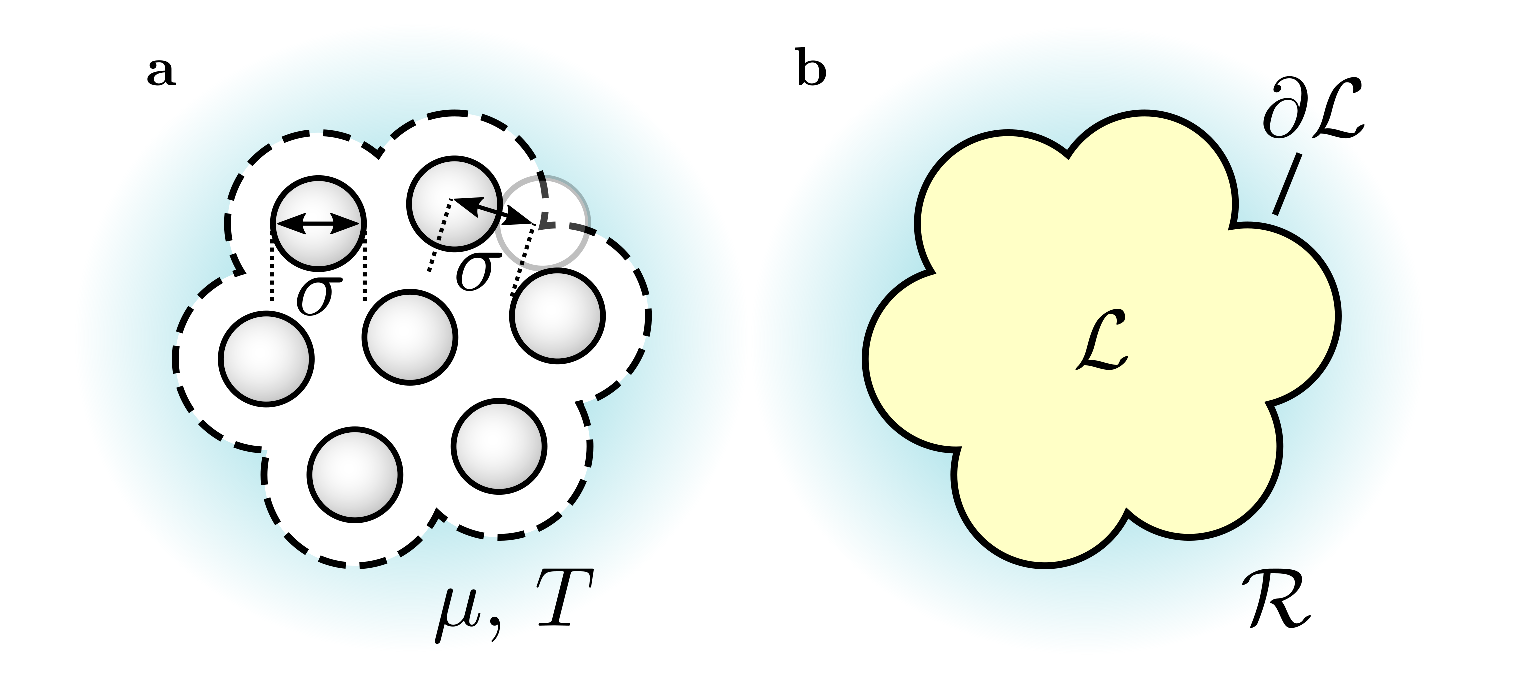
\includegraphics[width=\linewidth]{droplet-morph}
  \caption{
    The system considered showing
    (a) the local particles surrounded by the remaining liquid acting as a thermal reservoir at fixed chemical potential and temperature, and
    (b) partition of space into the local $\mathcal{L}$ and remaining $\mathcal{R}$ components with dividing surface $\partial\mathcal{L}$.
    In this work $\mathcal{L}$ is chosen as the space inaccessible to the centre of a test particle (shown faded) representing the remaining liquid.
  }
\end{SCfigure}

\subsection{Limitations known from DFT literature}
\subsection{As a generalisation of scaled particle theory}
And the limitations this implies.

\section{Worked examples where morphometric form can be exact}
Under certain conditions.
\subsection{Low density limit in arbitrary dimensions from lowest order terms in the virial expansion of the pressure}
\subsection{Arbitrary densities at large lengthscales}
\subsection{Hard rods (dimension d = 1) at all densities}
\subsubsection{Exact result from DFT}
\subsubsection{Morphometric result}
Explore where additivity, continuity and motion invariance apply.
\subsubsection{Implications for higher dimensions}

\section{Derivation of thermodynamic coefficients for hard spheres in $d = 3$}

\subsubsection{Scaled particle route}

We describe here in more detail the derivation of the first set of morphometric coefficients, equivalent to those given in \cite{Hansen-Goos2006} through fundamental measure theory (FMT).
The derivation sketched below avoids use of FMT, instead favouring a geometric formulation equivalent to the scaled particle approach of Reiss \emph{et al}.\ \cite{Reiss1959,Reiss1960}.
The standard scaled particle approach considers an expansion of the grand potential surrounding a spherical solute in powers of radii; here, we modify the \emph{ansatz} to use morphological measures instead, so that the resulting theory is more naturally extended to geometries of arbitrary shapes.
Additionally, we impose the Carnahan-Starling equation of state as an \emph{input} whereas the Percus-Yevick equation of state is an \textit{output} of standard scaled particle approaches.

Following the protocol of scaled particle theories, we consider the insertion of a hard ball of radius $R-\frac{\sigma}{2}$ into the liquid at the origin.
This choice of radius ensures that contact with the \emph{center} of solvent particles occurs at distance $R$ from the point of insertion i.e.\ $\rho(r) = 0$ for $r < R$.
Writing the change in the grand potential due to the insertion of the ball in its morphometric form (from \eqref{eq:surface-tension} and \eqref{eq:morphometric-surface-tension} of the main text), we have the \emph{ansatz}
\begin{equation}\label{eq:morph-ball-solvation}
  \Delta \Omega(R) =
  \frac{4\pi R^3}{3} p +
  4\pi R^2 \, \gamma_\infty +
  4\pi R \, \kappa +
  4 \pi \, \overline{\kappa}.
\end{equation}
If an equation of state for the pressure is taken as input, only three equations are needed to set the remaining coefficients of surface tension $\gamma_\infty, \kappa$ and $\overline{\kappa}$.

Restating the expressions for the insertion of a hard point and a new particle from the main text as
\begin{align}
  \label{eq:spt-point} \Delta\Omega(R=0) &= -k_B T \ln{(1- \eta)}, \\
  \label{eq:spt-mu} \Delta\Omega\left(R=\frac{\sigma}{2}\right) &= \mu^{ex},
\end{align}
we need one more equation to set the thermodynamic coefficients for the theory.
Following Ref.\ \cite{Bryk2003} we take the normal derivative of $\Omega$ with respect to $R$, and noting that $\Delta\Omega(R) = \Omega(R) - \Omega_{hom}$ gives
\begin{equation}\label{eq:spt-derivative}
  \left( \frac{\partial \Delta \Omega}{\partial R} \right)_{\mu,V,T} =
  \left( \frac{\partial \Omega}{\partial R} \right)_{\mu,V,T} =
  \int
  \frac{\delta \Omega[\rho_0(\vec{r})]}{\delta \rho}
  \left( \frac{\partial \rho_0(\vec{r})}{\partial R} \right)_{\mu,V,T}
  \, d\vec{r} +
  \int
  \rho_0(\vec{r})
  \left( \frac{\partial \phi_{ext}(\vec{r})}{\partial R} \right)_{\mu,V,T}
  \, d\vec{r},
\end{equation}
where $\rho_0$ is the equilibrium density profile and $\phi_{ext}$ is the external potential (i.e.\ the potential of the ball).
In equilibrium $\Omega$ is minimised so
\begin{equation}
  \left.
  \frac{\delta \Omega[\rho(\vec{r}); \phi_{ext}]}{\delta \rho}
  \right|_{\rho(\vec{r})=\rho_0(\vec{r})} = 0,
\end{equation}
so the first integral in \eqref{eq:spt-derivative} vanishes.
As the ball is hard, the external potential and its derivative are zero everywhere except at the surface $R$ where both $\rho_0$ and $\phi_{ext}$ are discontinuous.
We consider its Boltzmann weight, i.e.\
\begin{equation}
  e^{-\beta\phi_{ext}(\vec{r})} = \Theta(|\vec{r}| - R).
\end{equation}
Taking the derivative of both sides gives
\begin{equation}
  \beta\left( \frac{\partial\phi_{ext}(\vec{r})}{\partial R} \right)_{\mu,V,T} =
  \delta(|\vec{r}| - R) e^{\beta\phi_{ext}(\vec{r})}
\end{equation}
Inserting this expression into \eqref{eq:spt-derivative} and using the fact that $\rho(\vec{r}) e^{\beta\phi_{ext}(\vec{r})}$ is continuous (c.f.\ Ref.\ \cite{Hansen2013}) gives the contact theorem
\begin{equation}
  \beta \left( \frac{\partial \Omega}{\partial R} \right)_{\mu,V,T} =
  4\pi R^2 \rho(R).
\end{equation}
When $R = \sigma$ the inserted ball is equivalent to the hard sphere particles themselves, so $\Omega = \mu^{ex}$ and the contact density is $\rho(\sigma) = \rho \, g^{(2)}(\sigma)$ giving
\begin{equation}\label{eq:spt-contact-density}
  \left. \beta \left( \frac{\partial \Delta \Omega}{\partial R} \right)_{\mu,V,T}
  \right|_{R = \sigma}
  =
  \left. \beta \left( \frac{\partial \Omega}{\partial R} \right)_{\mu,V,T}
  \right|_{R = \sigma}
  =
  %\beta \frac{\partial \mu^{ex}}{\partial \sigma} =
  4\pi \sigma^2 \rho \, g^{(2)}(\sigma),
\end{equation}
or written in morphometric form using \eqref{eq:morph-ball-solvation} we have
\begin{equation}
  4\pi \sigma^2 \, p +
  8\pi \sigma \, \gamma_\infty +
  4\pi \, \kappa =
  \frac{4\pi \sigma^2 \rho}{\beta} \, g^{(2)}(\sigma).
\end{equation}
Applying the virial theorem (equation \eqref{eq:contact-g} in the main text) to the right hand side gives the final expression:
\begin{equation}\label{eq:spt-virial}
  4\pi \sigma^2 \, p +
  8\pi \sigma \, \gamma_\infty +
  4\pi \, \kappa =
  \frac{6}{\beta\sigma} \left( \frac{\beta p}{\rho} - 1 \right).
\end{equation}
Together \eqref{eq:spt-point}, \eqref{eq:spt-mu} and \eqref{eq:spt-virial} form a complete system of equations which we solve to obtain the coefficients
\begin{subequations}
  \begin{align}
    \frac{\beta \gamma_\infty^{WBII}}{R \rho} &=
    \left(\frac{\pi}{6\eta^2} - \frac{5\pi}{18\eta}\right) p -
    \frac{\mu^{ex}[p]}{3\eta} -
    \frac{\ln{(1-\eta)}}{3\eta} -
    \frac{1}{\eta}
    \label{eq:spt-gamma}
    \\
    \frac{\beta \kappa^{WBII}}{R^2\rho} &=
    \left( \frac{4\pi}{9\eta} - \frac{\pi}{2\eta^2} \right) p +
    \frac{4\mu^{ex}[p]}{3\eta} + \frac{4\ln{(1-\eta)}}{3\eta} + \frac{3}{\eta}
    \\
    \frac{\beta \overline{\kappa}^{WBII}}{R^3\rho} &=
    \left( \frac{\pi}{3\eta^2} - \frac{2\pi}{9\eta} \right) p -
    \frac{\mu^{ex}[p]}{\eta} - \frac{4\ln{(1-\eta)}}{3\eta} - \frac{2}{\eta}.
  \end{align}
\end{subequations}
Inserting the Carnahan-Starling parameters \eqref{eq:cs-pressure} and \eqref{eq:cs-mu} gives the coefficients explicitly as
\begin{subequations}
  \begin{align}
    \frac{\beta p^{WBII}}{\rho} &=
    \frac{1 + \eta + \eta^2 - \eta^3}{(1-\eta)^3}
    \\
    \frac{\beta \gamma_\infty^{WBII}}{R\rho} &=
    -\frac{1 + 2\eta + 8\eta^2 - 5\eta^3}{3(1-\eta)^3}
    - \frac{\ln{(1-\eta)}}{3\eta}
    \\
    \frac{\beta \kappa^{WBII}}{R^2\rho} &=
    \frac{4 - 10\eta + 20\eta^2 - 8\eta^3}{3(1-\eta)^3} + \frac{4 \ln{(1-\eta)}}{3\eta}
    \\
    \frac{\beta \overline{\kappa}^{WBII}}{R^3\rho} &=
    - \frac{4 - 11\eta + 13\eta^2 - 4\eta^3}{3(1-\eta)^3} - \frac{4 \ln{(1-\eta)}}{3\eta},
  \end{align}
\end{subequations}
which are \emph{identical} to the coefficients derived from the WBII free energy functional in Ref.\ \cite{Hansen-Goos2006}.
Remarkably, we have obtained these coefficients through a route completely different from their original derivation.
In Ref.\ \cite{Hansen-Goos2006} the coefficients were determined within FMT by taking the limit of a binary mixture where one component is infinitely dilute.
Here we completely avoided FMT, in favour of geometrical arguments similar to standard scaled particle approaches.
This suggests that the above scaled particle argument is somehow built into the structure of the WBII functional; we note that this is a nonobvious fact which cannot be determined from the form of the functional alone, nor is it obvious how it emerges from its original derivation.

Finally, note that (as described in the main text) the resulting $g^{(2)}$ performs poorly in the supercooled regime as compared with the ``exact'' result from virial theorem i.e.\ Eq.\ \eqref{eq:contact-g} in the main text.
In Fig.\ \ref{fig:contact-g} we plot the contact value with this set of coefficients, finding that it is reasonably accurate until around the freezing density where contact correlations spuriously decay.
The next section will detail how to modify the derivation to produce coefficients which describe more accurate correlation functions at high densities.

\begin{SCfigure}[h]
 \includegraphics[width=\linewidth]{g2_contact}
 \caption{
   Contact values of the radial distribution function against volume fraction $\eta$ and reduced pressure $Z = \beta p / \rho$ for the hard sphere liquid using Eq.\ \eqref{eq:contact-g} from the main text with Eq. \eqref{eq:g2-explicit} for the explicit form of $g^{(2)}$, assuming the Carnahan-Starling equation of state.
   Contact values are determined with two sets of morphometric coefficients: WBII (section \ref{sec:spt-route} and Ref.\ \cite{Hansen-Goos2006}) which performs poorly in the supercooled regime, and coefficients derived in this work (section \ref{sec:virial-route}) using the virial theorem which is exact by construction.
   The hard sphere freezing and melting volume fractions are indicated by vertical dashed lines.
   Inset: the errors $\Delta g = g^{(2)} - g^{(2)}_{MD}$ where $g^{(2)}_{MD}$ is determined from molecular dynamics simulations (c.f.\ section \ref{SI:molecular-dynamics}), showing the new theory also improves the accuracy away from contact.
   %\todo{Remove the inset and make that its own figure.}
 }
\label{fig:contact-g}
\end{SCfigure}

\subsection{Aside: scaled particle theory extension for dimers}

I was unaware of work by Stillinger et al \cite{Stillinger2006} before publishing on the morphometric approach, but upon discovering this work I realised their ideas are very similar in nature.
Here I present similar results but using the morphometric notation.%
\todo{The purpose of this section needs to be fleshed out and made \emph{very} clear, otherwise the reader will get lost quickly.
  This section \emph{is} important as we explore the boundaries of where the morphometric approach can fail: this is a great testbed for continuity, and allows us to argue the accuracy of the approach applied to local structures.}

We have the probability of any number of particles existing inside the cavity
\begin{equation}
  \sum_{n=0}^\infty p_n (\lambda) = 1
\end{equation}
Giving the probability the cavity is empty due to a spontaneous thermal fluctuation
as
\begin{equation}
  p_0 (\lambda) = e^{-\beta W(\lambda)}
  = 1 - \sum_{n=1}^\infty p_n (\lambda).
\end{equation}
The singular nature of the hard sphere interaction ensures there is a maximum number of particles that can fit inside any finite sized cavity (the optimal packing), so we define
\begin{equation}
  n^*(\lambda) = \max{n(\lambda)},
\end{equation}
and thus
\begin{equation}
  p_0 (\lambda) = e^{-\beta W(\lambda)}
  = 1 - \sum_{n=1}^{n^*(\lambda)} p_n (\lambda).
\end{equation}

Following Stillinger we generalise to two cavities.
Define work to insert both cavities as $W^{(2)}(r,\lambda)$.
We then have the generalisaton
\begin{equation}
  p_0^{(2)} (\lambda) = e^{-\beta W^{(2)}(\lambda)}
  = 1 - \sum_{n=1}^{\max{n^{(2)}(\lambda)}} p_n^{(2)} (\lambda).
\end{equation}
We have the conditions:%
\todo{Make this notation more consistent and able to handle different numbers of cavities. We don't want to just recycle Stillinger's notation: we want to be consistent with the rest of the thesis.}
\begin{align}
  \lim_{r \to 0} W^{(2)}(r; \lambda) &= W^{(1)}(\lambda) \\
  \max{n^{(2)}(r; \lambda)} &= 1
  \quad \forall \; r + 2\lambda < 1 \\
  \lim_{r \to \infty} W^{(2)}(r; \lambda) &= 2 W^{(1)}(\lambda) \\
  \max{n^{(2)}(r; \lambda)} &\le 2 \max{n^{(1)}(\lambda)}
  \quad \forall \; r > 2\lambda
\end{align}
\todo{Need to define $\lambda$ as the cavity diameter}[4cm]
Which gives us the `point' insertion condition (where $\max{n^{(2)}(r; \lambda)} = 1$)
\begin{equation}
  \beta W^{(2)}(r; \lambda) = -\ln (1 - \rho V(r; \lambda))
\end{equation}

Hausdorff distance is simply $r$, so how the hell is the Euler characteristic of their union continuous with respect to $r$? It is discontinuous at $r = 2\lambda$.

\subsubsection{Virial route}

In this section we give the detailed steps used in the derivation of the new set of morphometric coefficients, following the direction laid out in the main text.
In section \ref{SI:two-particles} above the morphological form of $g^{(2)}$ was computed explicitly; this derivation imposes the contact density using $\rho(\sigma) = \rho \, g^{(2)}(\sigma)$ with this explicit form.

From \eqref{eq:g2-explicit} the potential of mean force for neighbouring particles reduces to $\phi^{(2)}(r) = \Delta\Omega(r) - 2\mu^{ex}$ if they do not overlap, giving
\begin{equation}
  \begin{split}
  \phi^{(2)}(r) &\equiv - k_B T \ln g^{(2)}(r) \\
  &= pV(r) + \gamma_\infty A(r) + \kappa C(r) + \overline{\kappa} X(r) - 2\mu^{ex}
  \quad \forall \; \sigma \le r \le 2\sigma.
  \end{split}
\end{equation}
Inserting the morphological quantities at contact from \eqref{eq:g2-explicit-morph} gives
\begin{equation}
  \phi^{(2)}(\sigma) =
  \frac{9\pi \sigma^3}{4} p +
  6\pi\sigma^2 \, \gamma_\infty +
  \left( 6\pi\sigma - \frac{\pi^2\sigma}{2\sqrt{3}} \right) \, \kappa +
  4\pi \, \overline{\kappa}
  - 2\mu^{ex}[p].
\end{equation}
Equating this with $-k_B T \ln g^{(2)}(\sigma)$ and using the virial theorem (Eq.\ \eqref{eq:contact-g} in the main text) gives the final expression
\begin{equation}\label{eq:v-virial}
  \frac{9\pi \sigma^3}{4} p +
  6\pi\sigma^2 \, \gamma_\infty +
  \left( 6\pi\sigma - \frac{\pi^2\sigma}{2\sqrt{3}} \right) \, \kappa +
  4\pi \, \overline{\kappa} =
  2\mu^{ex}[p] - \beta^{-1} \ln{\frac{3}{2\pi \rho \sigma^3} \left( \frac{\beta p}{\rho} - 1 \right)}.
\end{equation}
We will use this last expression instead of the contact theorem \eqref{eq:spt-virial} in order to obtain new coefficients.
Together \eqref{eq:spt-point}, \eqref{eq:spt-mu} and \eqref{eq:v-virial} solve to give coefficients:
\begin{subequations}
  \begin{align}
    \frac{\beta \gamma_\infty^{V}}{R\rho} &=
    \frac{ (18\pi - 7\sqrt{3} \pi^2) p + 6\sqrt{3}\pi \mu^{ex}[p]
      - 6(12 - \sqrt{3}\pi) \ln{(1-\eta)}
      - 72\ln{\left( \frac{\pi p - 6\eta}{24\eta^2} \right)} }
    {54(\sqrt{3}\pi - 4) \eta}
    \label{eq:virial-gamma}
    \\
    \frac{\beta \kappa^{V}}{R^2\rho} &=
    \frac{ 5\pi p - 12 \mu^{ex}[p] + 24 \ln{(1-\eta)}
      + 36\ln{\left( \frac{\pi p - 6\eta}{24\eta^2} \right)} }
    {9(\sqrt{3}\pi - 4) \eta}
    \\
    \frac{\beta \overline{\kappa}^{V}}{R^3\rho} &=
    - \frac{
      (18\pi - 2\sqrt{3} \pi^2) p - (36 - 3\sqrt{3}\pi) \mu^{ex}[p] + 12\sqrt{3}\pi \ln{(1-\eta)}
      + 72\ln{\left( \frac{\pi p - 6\eta}{24\eta^2} \right)} }
    {27(\sqrt{3}\pi - 4) \eta},
  \end{align}
\end{subequations}
which upon insertion of the Carnahan-Starling parameters \eqref{eq:cs-pressure} and \eqref{eq:cs-mu} gives the coefficients explicitly as
\begin{subequations}
  \begin{align}
    \frac{\beta p^{V}}{\rho} &=
    \frac{1 + \eta + \eta^2 - \eta^3}{(1-\eta)^3} \\
    \frac{\beta \gamma_\infty^{V}}{R\rho} &=
    \frac{ 18\eta \frac{1 + \eta + \eta^2 - \eta^3}{(1-\eta)^3}
      + \sqrt{3}\pi\eta \frac{1 - 16\eta - 4\eta^2 + 7\eta^3}{(1-\eta)^3}
      - (12 - \sqrt{3}\pi) \ln{(1-\eta)}
      - 12\ln{\left( \frac{2 - \eta}{2(1-\eta)^3} \right)} }
    {9(\sqrt{3}\pi - 4) \eta} \\
    \frac{\beta \kappa^{V}}{R^2\rho} &= -
    \frac{ 2\eta \frac{11 - 23\eta + \eta^2 + 5\eta^3}{(1-\eta)^3}
      - 8 \ln{(1-\eta)}
      - 12\ln{\left( \frac{2 - \eta}{2(1-\eta)^3} \right)} }
    {3(\sqrt{3}\pi - 4) \eta} \\
    \frac{\beta \overline{\kappa}^{V}}{R^3\rho} &=
    \frac{ 12\eta \frac{5 - 12\eta + 3\eta^3}{(1-\eta)^3}
      - \sqrt{3}\pi\eta \frac{4 - 13\eta - \eta^2 + 4\eta^3}{(1-\eta)^3}
      - 4\sqrt{3}\pi \ln{(1-\eta)}
      - 24\ln{\left( \frac{2 - \eta}{2(1-\eta)^3} \right)} }
    {9(\sqrt{3}\pi - 4) \eta}.
  \end{align}
\end{subequations}
Unlike the WBII coefficients above these are entirely new, and produce significantly more accurate correlation functions at high densities as described in the main text.
The pair correlation produced by these coefficients (black line in Fig.\ \ref{fig:contact-g}) is self-consistent with CS at contact by construction, but as an additional bonus we find that the new coefficients provide a theory that outperforms the older WBII approach across the whole range of distances typical of neighbouring particles (inset of Fig.\ \ref{fig:contact-g}).
The latter observation enables us to accurately model complex many-particle local structures.

However, it should be noted that the planar surface tension $\gamma_\infty^{V}$ is considerably less accurate than $\gamma_\infty^{WBII}$ as compared with molecular dynamics studies in \cite{Davidchack2016}.
For this reason, WBII coefficients may give more accurate grand potentials (and thus correlations) for large solutes where the surface becomes approximately planar.

\section{Accuracy of predicted distribution functions in $d = 3$}

\begin{SCfigure}[h]
 \includegraphics[width=\linewidth]{g2_phi045}
 \caption{$g^{(2)}(r)$ for $\eta = 0.45$.}
\end{SCfigure}

\subsection{Comparison with molecular dynamics simulations}
\subsection{Comparison with Kirkwood superposition approximation}

\end{document}
